\section{Introduzione}
\rhead{Introduzione}
In questa sezione vengono analizzate brevemente ed in maniera informale le funzionalità offerte e l'architettura della soluzione.
\subsection{Requisiti funzionali informali}
\label{reqinf}
Lo strumento offre le seguenti funzionalità: 
\begin{itemize} [nosep]
\smallskip
\item  [\emph{Fu.1}]\textbf{Offuscamento dei dati} \newline
Il tool offre la possibilità di applicare le tecniche di offuscamento e restituire le tuple offuscate. 

\smallskip
\item  [\emph{Fu.2}]\textbf{Automazione dei test} \newline
Il tool offre la possibilità di eseguire automaticamente test parametrici su applicazioni Android. Lo strumento è inoltre in grado di catturare il risultato dei test e, in base a questo, verificare se il bug atteso è stato riprodotto. Sono inoltre offerte le seguenti funzionalità secondarie:
	\begin{itemize} [nosep]	
			\item Salvataggio di uno screenshot per ogni test lanciato
		\item Salvataggio di uno screen record per ogni test lanciato
	\end{itemize}

\smallskip
\item  [\emph{Fu.3}]\textbf{Offuscamento dei dati + Automazione dei test} \newline
Il tool offre la possibilità di utilizzare in sequenza le funzionalità precedenti permettendo il raggiungimento dell'obiettivo dello stage. E' possibile infatti eseguire automaticamente test parametrici utilizzando in input le tuple offuscate ottenute applicando le tecniche di offuscamento sui dati originali che provocano il bug. In questo modo lo strumento è in grado di verificare, per ogni tupla offuscata, se il bug atteso (provocato dalla tupla non offuscata) è stato riprodotto.
%\medskip
\end{itemize}  

\noindent Risulta opportuno evidenziare che il tool è orientato a quest'ultima funzionalità  in quanto è quella che permette il raggiungimento dell'obiettivo per cui è stato creato.  

%Quindi,  le funzionalità di solo offuscamento dei dati e di solo automazione dei test 


\subsection{Architettura della soluzione}
La soluzione adottata, in grado di offrire le funzionalità identificate nella sezione precedente (Sezione \ref{reqinf}), segue il modello esposto nella Figura  \ref{fig:archsol}.
\begin{figure}[H]
	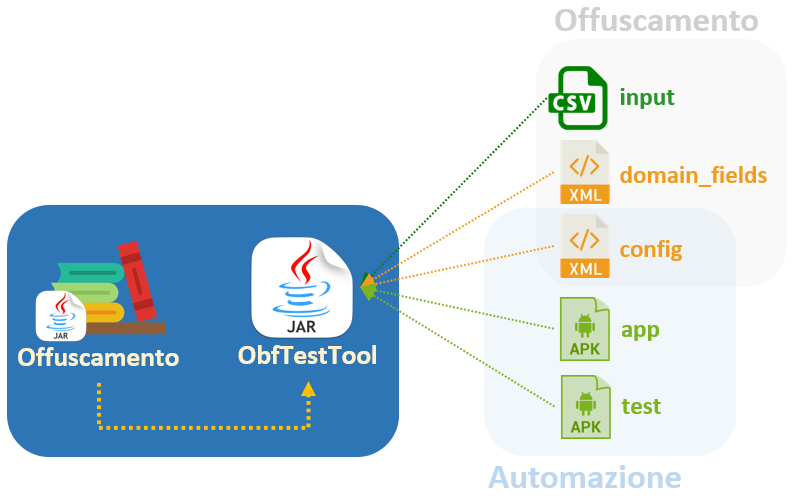
\includegraphics[scale=0.60]{architettura.della.soluzione}
	\centering
	\caption{Architettura della soluzione}%\footnote{Immagine realizzata da A. Belisario}
    \label{fig:archsol}
\end{figure}
\noindent Il tool è stato impacchettato in un file JAR (\emph{ObfTestTool}) lanciabile da linea di comando, che utilizza la libreria di offuscamento (\emph{Offuscamento}) citata nella Sezione \ref{liboff}.  Come evidente nella Figura \ref{fig:archsol}, lo strumento necessita di alcuni file di configurazione  (\emph{domain\_fields.xml}, \emph{config.xml}) e di alcuni file di input  (\emph{input.csv}, \emph{app.apk}, \emph{test.apk}) in maniera differente in base alla funzionalità che si vuole sfruttare.